\section{Historia sieci Tor}
Sieć Tor powstawała przez wiele lat. Początkowo był to projekt rządowy, mający na celu ochronę komunikacji wywiadowczej Stanów Zjednoczonych, lecz na przestrzeni lat stał się wolnym, dostępnym publicznie oprogramowaniem\footnote{https://www.onion-router.net/History.html\label{hist}}\footnote{J. B. Fagoyinbo, The Armed Forces: Instrument of Peace, Strength, Development and Prosperity, Bloomington 2013, s. 262}. 

Rozwój sieci Tor można podzielić na kilka generacji. Od momentu rozpoczęcia prac w~1995 roku do wydania oprogramowania w~połowie 1996 roku trwał pierwszy etap rozwoju projektu. Po niej, a~przed pojawieniem się sieci Tor, trwał etap nazywany Trasowanie Cebulowe: Następna Generacja (ang. Onion Routing: The Next Generation). Ostatni etap rozwoju, trwający aż do teraz nosi nazwę "Tor: The Second-Generation Onion Router", chociaż przyjęło mówić się po prostu Tor (The Onion Router). Ze względu na to, że ostatni etap rozwoju sieci Tor wskazuje, że jest to druga generacja, więc numerację należy zacząć od 0. Tak więc pierwszy etap będzie generacją 0, drugi generacją 1, a ostatni oczywiście generacją 2\footnote{\url{https://www.onion-router.net/}\label{onionrouter}}.

Obecnie rozwojem i~utrzymaniem sieci Tor zajmuje się organizacja non-profit The Tor Project, założona w~2006 roku\footnote{https://www.torproject.org/press/2008-12-19-roadmap-press-release}.

\subsection{Generacja 0}
Prowadzenie pierwszych rozmów na temat Trasowania Cebulowego rozpoczęto w~1995 roku. Początkowo dyskusje dotyczyły funkcji, które ma posiadać i~na jakiej zasadzie ma ono działać. Projekt został sfinansowany przez Biuro ds. Badań i~Rozwoju Marynarki Wojennej (ONR)\textsuperscript{\ref{hist}}.

Rok później pojawiła się już pierwsza formalna publikacja, oraz prezentacja Trasowania Cebulowego pod nazwą "Hiding Routing Information". Została ona opublikowana na First Hiding Workshop 31 Maja. Zostały w~niej m.in. cel powstania Trasowania Cebulowego, zasada działania, a~także podatności na pewne rodzaje ataków. Trasowanie Cebulowe było odporne na analizę ruchu w~czasie rzeczywistym, lecz jednak po zebraniu odpowiedniej liczby danych możliwe było odkrycie stron komunikacji. Także przejęcie pierwszego, inicjującego serwera proxy sprawiało, że wszystkie dane były ujawnione\footnote{https://www.onion-router.net/Publications/IH-1996.pdf\label{hri}}.

W~tym samym roku został uruchomiony pierwszy działający prototyp projektu, składający się z~5~węzłów działających na maszynie z~systemem Solaris 2.5.1/2.6, znajdującej się w~Laboratorium Badań Morskich (NRL)\textsuperscript{\ref{hist}}. Działająca wersja posiadała wsparcie dla protokołów HTTP, oraz Telnet, jednakże trwały prace nad serwisami mogącymi działać także z~protokołami FTP i~SMTP\textsuperscript{\ref{hri}}.

\subsection{Generacja 1}
Jeszcze tego samego roku rozpoczęto prace nad Trasowaniem Cebulowym 1.~generacji, zwanego również Systemem Następnej Generacji (ang. Next Generation System)\textsuperscript{\ref{onionrouter}}. Prace obejmowały m.in. usunięcie z~głównej części kodu, fragmentu odpowiedzialnego za kryptografie, co miało zapewnić większą modułowość. Zdecydowano się również na zachowanie projektu w~postaci otwartoźródłowej. Dzięki publicznie dostępnemu kodowi źródłowemu Trasowanie Cebulowe zapewniłoby większe bezpieczeństwo. Każda luka mogła być bardzo szybko zauważona przez społeczność i~naprawiona. Sprawiało to również, że oprogramowanie było darzone większym zaufaniem. Użytkownik nie musiał bać się o~swoją anonimowość, wierząc twórcom oprogramowania na słowo, że w~kodzie nie znajduje się fragment, który ujawnia dane zawieracjące inforamcje o~jego tożsamości. Miało to zachęcić większą liczbę osób chcących zapobiec analizie ruchu sieciowego przesyłanych przez siebie wiadomości do korzystania właśnie z~Trasowania Cebulowego. Kolejnym powodem dla którego zdecydowano się tworzyć projekt o~otwartym kodzie były pewne ograniczenia eksportowe, które uniemożliwiały rozpowszechnienie kodu Trasowania Cebulowego generacji 0. W~Lipcu uznano, że kod projektu może zostać udostępniony publicznie.

W~1997 roku projekt Trasowania Cebulowego,  w~ramach Programu High Confidence Network, dostał wsparcie finansowe od Agencji Zaawansowanych projektów Badawczych w~Obszarze Obronności (DARPA). Tego samego roku Trasowanie Cebulowe otrzymało wiele nowych funkcjonalności, m.in. od tego momentu ścieżka, po której były przesyłane pakiety, mogła posiadać zmienną długość, routery zostały oddzielone od serwerów proxy, a~moduł kryptograficzny mógł zostać uruchomiony na oddzielnej, specjalnie do tego przeznaczonej maszynie. 

Rok później organizacje NRL, NRAD, oraz UMD zdecydowały się na uruchomienie, w~swoich oddziałach, kilku sieci Trasowania Cebulowego. Były to implementacje zarówno generacji~0, jak i~1. Zbudowane sieci mogły obsłużyć protokoły HTTP, FTP, SMTP, oraz rlogin\textsuperscript{\ref{hist}}. 

Pod koniec tego samego roku organizacja Zero Knowledge Systems ogłosiła, powstanie własnej sieci - Freedom Network, o podobnym działaniu co Trasowanie Cebulowe. Projekt ten składał się z~komercyjnych węzłów pośredniczących, a~nie tak jak w~Trasowaniu Cebulowym z węzłów utrzymywanych przez ochotników. Użytkownicy którzy chcieli korzystać z~tego sposobu zachowania anonimowości, musieli wykupić subskrybcję. Jednakże projekt ten nie zdołał się zbyt długo utrzymać. Już pod koniec 2001 roku sieć została zamknięta. Rozwiąznanie to nie cieszyło na tyle dużą popularnością, aby organizacja była w~stanie pokryć kosztów utrzymania swoich węzłów pośredniczących.

W~1999 roku publikacja dotycząca Trasowania Cebulowego o~nazwie "Anonymous Connection and Onion Routing" została nagrodzona nagrodą Alan Berman Research Publication Award. Nagroda ta została ustanowiona przez pracownika NRL - Dr. Alana Bermana i~przyznawana jest za najlepsze pisma techniczne w~każdej z~dziedzin naukowych\footnote{https://www.gl.ciw.edu/news/ahart-receives-berman-award}. Mimo to prace nad projektem zostały tymczasowo wstrzymane, aczkolwiek prace badawcze i~analityczne nadal trwały.

Kolejnego roku została zamknięta jedna z~prototypowych sieci generacji 0. W~trakcie swojego 2-letniego działania zanotowano ponad 20 milionów zapytań z ponad 60 krajów. Maksymalne obciążenie wyniosło 84022 odwiedzin i~zostało odnotowane 12 grudnia 1998 roku. Wykres przedstaiający dzienne użycie sieci testowej w~NRL został przedstawiony na rysunku \ref{rys:dzienny}.

\begin{figure}
  \centering
  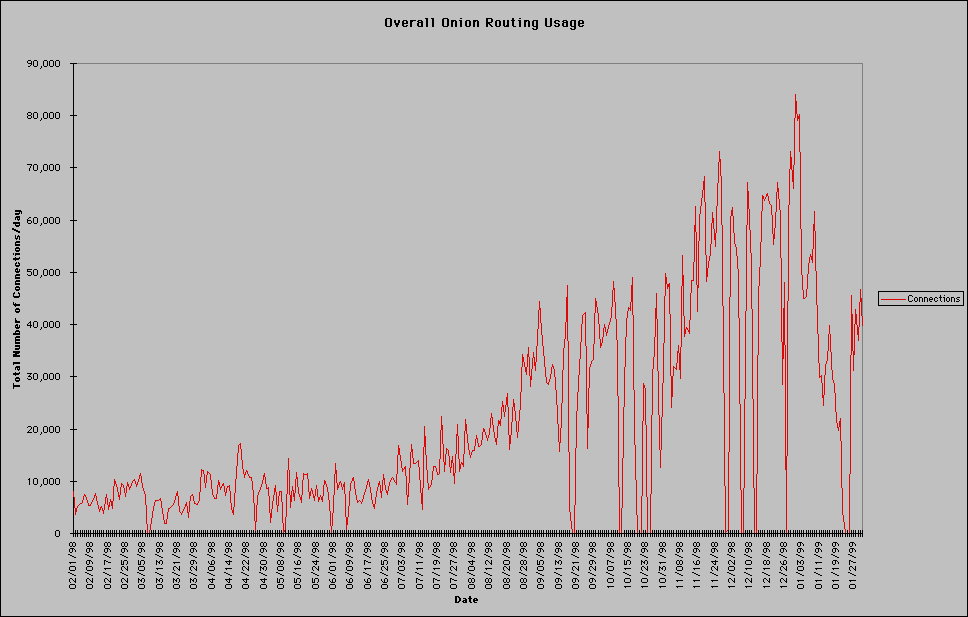
\includegraphics[width=\textwidth]{Daily} 
  \caption[Caption for LOF]{Dzienny przepływ ruchu w~prototypowej sieci w~NRL\footnotemark.}
  \label{rys:dzienny}
\end{figure}
\footnotetext{https://www.onion-router.net/Archives/Daily.gif}

Po dwuletniej przerwie w~rozwoju ponowiono pracę nad rozwojem Trasowania Cebulowego. Projekt został sfinansowany przez DARPA w~ramach programu Fault Tolerant Networks.

\subsection{Generacja 2}
Rok 2002 był przełomowy dla projektu. Cały dotychczasowy kod został porzucony, ze względu na swoją przestarzałość. Projekt został napisany od nowa. Jako bazę dla nowej wersji Trasowania Cebulowego wykorzystano projekt jednego ze studentów uniwersytetu w~Cambridge - Mateja Pfajfara. Od czasu rozpoczęcia prac nad Trasowaniem Cebulowym minęło 6 lat. W~tym czasie powstały niezależne filtrujące serwery proxy, będące w~stanie sprostać wymaganiom projektu. Do tego celu wykorzystano Privoxy. Pośredniczeniem na poziomie warstwy aplikacji miał zajmować się protokół SOCKS. Był on wstanie obsługiwać większość protokołów, którymi obsługą miało zajmować się Trasowanie Cebulowe. Dzięki temu pracownicy nie musieli się już zajmować rozwojem oprogramowania dla serwerów proxy każdej z~aplikacji. 

W~2003 roku Tor otrzymał wsparcie finansowe od ONR, DARPA i~NRL. Tego samego roku została uruchomiona pierwsza sieć Trasowania Cebulowego 2. generacji. Od samego początku działania sieci zaczęli pojawiać się nowi ochotnicy chcący rozwijać projekt przez udostępnienie swoich maszyn jako węzłów pośredniczących sieci Tor, początkowo tylko z~USA, lecz później do projektu dołączyli ochotnicy z~innych krajów. 

Rok później zostały uruchomione pierwsze ukryte serwisy, oraz ukryta wiki (Hidden Wiki). 13. Sierpnia Tor został przedstawiony na USENIX Security jako "Tor: Second-Generation Onion Router". Pod koniec roku ONR i~DARPA zakończły wsparcie finansowe projektu, ale zamiast nich finansowanie rozwoju i~wdrażania projektu rozpoczął EFF\textsuperscript{\ref{hist}}.

\subsection{Projekt Tor}
W~Grudniu 2006 roku została założona ogranizacja non-profit The Tor Project. Miała ona na celu zapewnić dalszy rozwój, oraz utrzymanie sieci Tor. Wśród jej twórców znajdują się m.in. Roger Dingledine i~Nick Mathewson\footnote{https://www.torproject.org/about/findoc/2009-TorProject-Form990andPC.pdf}. Początkowo sponsoringiem fiskalnym The Tor Project zajmowała się, założona w~1990 roku pozarządowa organizacja Electronic Frontier Foundation (EFF), której głównym celem jest walka o~wolność słowa, oraz prywatności w Internecie\footnote{\url{https://www.eff.org/about}}\footnote{\url{https://www.eff.org/press/archives/2004/12/21-0}}. Wsparciem finansowym projektu zajmowali się takie organizacje jak: Broadcasting Board of Governors, National Science Foundation, Internews Europe, Human Rights Watch, Cyber-TA project, Bell Security Solutions, a także Omidyar Network Enzyme Grant\footnote{\url{https://www.torproject.org/about/sponsors.html.en}}.

The Tor Project, oprócz rozwoju Tor, zajmuje się również tworzeniem oprogramowania, które ma zapewnić anonimowość w Internecie przy wykorzystaniu sieci Tor. Flagowym projektem jest Tor Browser. Jest to przeglądarka internetowa, bazująca na Mozilli Firefox, zawieracjąca wbudowanego klienta sieci Tor. Używając jej do przeglądania stron internetowych, cały nasz ruch jest szyfrowany, a~następnie przekierowywany przez sieć Tor. Dzięki niej mamy również umożliwiony dostęp do ukrytych stron internetowych, korzystających ze specjalnej, używanej tylko w~sieci Tor, domeny najwyższego poziomu .onion\footnote{\url{https://www.torproject.org/projects/torbrowser/design/}}. Przeglądarka została publicznie udostępniona na oficjanlej stronie The Tor Project w~2008 roku\footnote{\url{https://web.archive.org/web/20081029125231/http://www.torproject.org:80/easy-download.html.en}}. Była ona dostępna pod nazwą Tor Browser Bundle, a~od 2014 roku nosi po prostu nazwę Tor Browser\footnote{\url{https://web.archive.org/web/20140701221249/https://www.torproject.org/projects/torbrowser.html.en}}. Do innych ważniejszych projektów organizacji The Tor Project można zaliczyć Orbot~-~aplikację wydaną w~2008 roku, przeznaczoną na system operacyjny Android, której celem jest szyfrowanie, a~następnie przekierowywanie przez sieć Tor przesyłanych przez Internet danych, wybranych przez użytkownika aplikacji znajdujących się na urządzeniu\footnote{\url{https://guardianproject.info/apps/orbot/}}. W~2009 roku została wydana pierwsza wersja programu działającego w~trybie tekstowym o~nazwie Nyx\footnote{\url{https://nyx.torproject.org/changelog/legacy.html}}. Została ona przeznaczona dla osób, które chciałyby monitorować stan administrowanego przez siebie przekaźnika znajdującego się w~sieci Tor. Program ten został napisany w~języku Python i~pozwala m.in. na obserwację wykorzystania zasobów komputera, nawiązanych połączeniach i~wielu innych informacji o~naszym przekaźniku\footnote{https://www.torproject.org/projects/nyx.html.en}. Poza powyżej wymienionymi jest jeszcze wiele innych aplikacji, pomagających w~ochronie naszej prywatności, przy wykorzystaniu sieci Tor\footnote{https://www.torproject.org/projects/projects.html.en}.

Dzięki swoim osiągnięciom w~walce o~zachowanie anonimowości, prywatności i~wolności słowa w~Internecie The Tor Project otrzymał wiele nagród. Wśród nich można wyróżnić Free Software Foundation 2010, otrzymaną w~Marcu 2011 roku za Projects of Social Benefit. Nagroda ta przyznawana jest projektom, które przynoszą korzyści dla społeczeństwa\footnote{\url{https://www.fsf.org/news/2010-free-software-awards-announced}}. Z~kolei we Wrześniu 2012 roku Projektowi Tor została przyznana EFF Pioneer Award, która zostaje przyznawana od 1992 roku liderom, którzy wpływają na rozwój wolności, oraz innowacji w~zakresie technologii informatycznych\footnote{\url{https://www.eff.org/awards/pioneer/2012}}.